\documentclass[11pt,a4paper]{article}

%
% Packages
%
\usepackage[T1]{fontenc} % Output font encoding for international characters
\usepackage[utf8]{inputenc} % Required for inputting international characters
\usepackage{amsmath,amsthm,amssymb}
\usepackage[svgnames]{xcolor}
\usepackage[english,french]{babel}
\usepackage{multicol}
\usepackage{pstricks,pst-node,pst-text,pst-poly,pst-3d}
\usepackage{enumitem}
\usepackage{sidenotes}
\usepackage{graphicx} % Required to insert images
\usepackage{array}
\usepackage{booktabs} % Required for better horizontal rules in tables
\usepackage{titlesec} % Required for modifying sections
\usepackage{tikz}
\usetikzlibrary{trees}
\usepackage{verbatim}

%
% Constant and Variables
%
\setlength{\textwidth}{175mm}
\setlength{\textheight}{255mm}
\setlength{\oddsidemargin}{-10mm}
\setlength{\topmargin}{-15mm}
\setlength{\parskip}{0.2cm}
\definecolor{vertfonce}{rgb}{0,0.5,0}
% Set the overall layout of the tree
\tikzstyle{level 1}=[level distance=3.5cm, sibling distance=3.5cm]
\tikzstyle{level 2}=[level distance=3.5cm, sibling distance=2cm]
% Define styles for bags and leafs
\tikzstyle{bag} = [text width=4em, text centered]
\tikzstyle{end} = [circle, minimum width=3pt,fill, inner sep=0pt]

%
% Custom commands
%

\newcommand{\ds}{\displaystyle}
\newcommand{\scr}{\scriptscriptstyle}
\newcommand{\bs}[1]{\ensuremath{\boldsymbol{#1}}}

%
% Header
%
\newcommand{\header}[2]{

\noindent {\sc HEIG--VD} \hfill Probabilités et Statistique\newline 
\noindent {Corrigé Etudiant} \hfill 2021-2022\newline
\hrule
\vspace{3mm}
\noindent {\bf Thème : #1} \hfill Solution de la #2
\vspace{5mm}
\hrule
\vspace{7mm}
}
%

%
\newcommand{\separation}{{\begin{center}\rule{10cm}{0.25pt}\end{center}}\noindent} % crée une barre
%

%
% Math
%
\newcommand{\Real}{\mathbb R}
\newcommand{\RPlus}{\Real^{+}}
\newcommand{\norm}[1]{\left\Vert#1\right\Vert}
\newcommand{\abs}[1]{\left\vert#1\right\vert}
\newcommand{\setn}[1]{\left\{#1\right\}_{\scriptscriptstyle n \ge 1}}
\newcommand{\set}[1]{\left\{#1\right\}}
\newcommand{\seq}[1]{\left<#1\right>}
\newcommand{\eps}{\varepsilon}
\newcommand{\To}{\longrightarrow}
\newcommand{\Prob}{\rm{P}}
\newcommand{\F}{\mathcal{F}}
\newcommand{\h}{\mathcal{H}}
\newcommand{\M}{\mathcal{M}}
\newcommand{\X}{\mathcal{X}}
\newcommand{\N}{\mathcal{N}}
\newcommand{\E}{{\rm E}}
\newcommand{\Hnull}{{\rm H}_{0}}
\newcommand{\Hone}{{\rm H}_{1}}
\newcommand{\Var}{{\rm Var}}
\newcommand{\Cov}{{\rm Cov}}
\newcommand{\sign}{{\rm sign}}
\newcommand{\med}{{\rm med}}
\newcommand{\tr}{{\rm tr}}
\newcommand{\T}{{\text{\tiny \rm T}}}
\newcommand{\minf}{- \, \infty}
\newcommand{\intervalle}[4]{\mathopen{#1}#2\mathpunct{},#3\mathclose{#4}}
\newcommand{\intervalleff}[2]{\intervalle{[}{#1}{#2}{]}}
\newcommand{\intervalleof}[2]{\intervalle{]}{#1}{#2}{]}}
\newcommand{\intervallefo}[2]{\intervalle{[}{#1}{#2}{[}}
\newcommand{\intervalleoo}[2]{\intervalle{]}{#1}{#2}{[}}
\newcommand*\conj[1]{\overline{#1}}
\newcommand*\mean[1]{\overline{#1}} 

%
% Section
%
\titleformat
{\section} % Section type being modified
[block] % Shape type, can be: hang, block, display, runin, leftmargin, rightmargin, drop, wrap, frame
{\Large\bfseries} % Format of the whole section
{\assignmentQuestionName~\thesection} % Format of the section label
{6pt} % Space between the title and label
{} % Code before the label
\titlespacing{\section}{0pt}{0.5\baselineskip}{0.5\baselineskip} % Spacing around section titles, the order is: left, before and after

%
% Subsection
%
\titleformat
{\subsection} % Section type being modified
[block] % Shape type, can be: hang, block, display, runin, leftmargin, rightmargin, drop, wrap, frame
{} % Format of the whole section
{\alph{subsection})} % Format of the section label
{4pt} % Space between the title and label
{} % Code before the label
\titlespacing{\subsection}{0pt}{0.5\baselineskip}{0.5\baselineskip} % Spacing around section titles, the order is: left, before and after


%
%	Custom Exercice Environnment
%------------------------------------------------
\newcommand{\assignmentQuestionName}{Exercice} % The word to be used as a prefix to question numbers

% Environment to be used for each question in the assignment
\newenvironment{exo}{
	\vspace{0.5\baselineskip} % Whitespace before the question
	\section{} % Blank section title (e.g. just Exercice 2)
}

% Command to print a question sentence
\newcommand{\donnee}[1]{
	\noindent{Donnée: }
	\emph{#1}
	\vspace{0.5\baselineskip} % Whitespace afterwards
}

% Environment for subexercice, takes 1 argument - the name of the section
\newenvironment{subexo}[1]{
	\subsection{\itshape{#1}}
}

% Command to print a box that breaks across pages with the question answer
\newcommand{\answer}[1]{#1}
%------------------------------------------------

\frenchspacing

\graphicspath{ {./} }


\begin{document}
	\header{probabilités élémentaires}{Série 1}
	%
	% Exercice 1
	%
	\begin{exo}
		\donnee{Un groupe de consommateurs a réalisé une étude pour analyser le service offert par 200 employés de	divers restaurants. On s’intéresse à une possible relation entre la qualité du service et la qualification du personnel (diplômé d’une école hôtelière ou non). Les résultats de l’enquête figurent dans le tableau ci-dessous : 
			\begin{center}
				\begin{tabular}{lll}
					& Bon service & mauvais service \\
					\toprule
					Diplôme & 61 & 28 \\
					\midrule
					Sans diplôme & 30 & 81 \\
					\bottomrule
				\end{tabular}
			\end{center}}
		Rappel : $P(A) = \frac{\text{Nombre de cas favorables}}{\text{Nombre de cas possibles}}$
		\begin{subexo}{Calculer les probabilités d’avoir choisi une personne :}
		\begin{enumerate}[parsep=0cm, itemsep=3mm, topsep=3mm]
			\item dont le service est qualifié bon.
			\begin{enumerate}
				\item[ ] \text{Ici on réunis les bons services des personnes avec et sans diplôme. On a donc : } 
				\item[ ] \begin{center}{Cas fav.} = 61 + 30 = 91\end{center} 
				\item[ ] \text{Ensuite on calcul les cas possibles. On a donc : } 
				\item[ ] \begin{center}{Cas tot.} = 61 + 28 + 30 + 81 = 200\end{center} 
				\item[ ] \text{On applique la formule et on obtient : } 
				\item[ ] \begin{center}$\dfrac{91}{200} = 0,455$\end{center} 
			\end{enumerate}
			\item non diplômée.
			\begin{enumerate}
				\item[ ] \text{Ici on réunis les personnes sans diplôme, peut importe la qualité du service. On a donc : } 
				\item[ ] \begin{center}{Cas fav.} = 30 + 81 = 111\end{center} 
				\item[ ] \text{Ensuite on calcul les cas possibles. On a donc : } 
				\item[ ] \begin{center}{Cas tot.} = 61 + 28 + 30 + 81 = 200\end{center} 
				\item[ ] \text{On applique la formule et on obtient : } 
				\item[ ] \begin{center}$\dfrac{111}{200} = 0,555$\end{center} 
			\end{enumerate}
			\item diplômé dont le service est bon.
			\begin{enumerate}
				\item[ ] \text{Ici on réunis les personnes avec diplôme et une bonne qualité de service. On a donc : } 
				\item[ ] \begin{center}{Cas fav.} = 61\end{center} 
				\item[ ] \text{Ensuite on calcul les cas possibles. On a donc : } 
				\item[ ] \begin{center}{Cas tot.} = 61 + 28 + 30 + 81 = 200\end{center} 
				\item[ ] \text{On applique la formule et on obtient : } 
				\item[ ] \begin{center}$\dfrac{61}{200} = 0,305$\end{center} 
			\end{enumerate}
		\end{enumerate}
		\end{subexo}
		\begin{subexo}{Quelle hypothèse faites-vous pour déterminer ces probabilités ?}
			Toutes les probabilités sont \textbf{équiprobables}. C'est pour cela qu l'on peut utiliser la formule énnoncée dans les rappels de l'exercice.
			
		\end{subexo}
	\end{exo}
	%
	% Exercice 2
	%
	\begin{exo}
		\donnee{Sur le chemin de l’école, un étudiant de la HEIG–VD s’arrête toujours à la même station-service pour faire le plein d’essence. Il a constaté que les deux pompes de la station notées A et B ont la même probabilité d’être occupées. De plus, la probabilité que l’une des deux pompes au moins soit utilisée vaut 0.9 et celle que toutes les deux soient simultanément occupées est 0.5.}

		Pour faciliter la compréhension de cet exercice, on peut réaliser un diagramme de Venn.
		\begin{center}\includegraphics[scale=0.5]{ex2-diagrammeVenn}\end{center}
		Premièrement, posons que :
		\begin{multicols}{4}
			\begin{enumerate}[label=\alph*), parsep=0cm, itemsep=3mm, topsep=3mm]
				\item[ ] AO = La pompe A est occupée
				\item[ ] AL = La pompe A est libre
				\item[ ] BO = La pompe B est occupée
				\item[ ] BL = La pompe B est libre
			\end{enumerate}
		\end{multicols}
		\begin{center}$\Omega = \{(AL,BL),(AO,BL),(AL,BO),(AO,BO)\}$ \text{, évènements pas équiprobable !!!}\end{center}
		On sait que les probabilités que A soit libre sont les mêmes pour B. On note :
		\begin{center}$P(\{AL\}) = P(\{BL\})$\end{center}
		On sait aussi que :
		\begin{enumerate}
			\item[ ] $P(\text{au moins une pompe soite occupée}) = 0.9$
			\item[ ] $P(\text{les deux pompes soient occupées}) = 0.5$
			\item[ ] $P(\Omega) = 1$
		\end{enumerate}
		\begin{subexo}{Calculer la probabilité que les deux pompes soient disponibles.}
			Parmis les évènements probables on sait que : 
			\begin{center}$P\{(AO,BL),(AL,BO),(AO,BO)\} = 0.9$\end{center}
			Puisque nous cherchons la probabilité du couple manquant $(P\{(AL,BL)\})$, on pose :
			\begin{center}$P(\Omega) = P\{(AL,BL)\} + P\{(AO,BL),(AL,BO),(AO,BO)\}$\end{center}
			En remplaçant les probabilités connues par leurs valeurs, on obtient :
			\begin{center}$1 = P\{(AL,BL)\} + 0.9$\end{center}
			On peut donc en conclure que $P\{(AL,BL)\}  = 0.1$ et donc que la probabilité que la pompe A et B soient libre est de $0.1$
		\end{subexo}
	\begin{subexo}{Déterminer la probabilité que la pompe A soit libre.}
		Rappel : $P(A\cup B) = P(A) + P(B) - P(A \cap B)$ \\ \\ 
		Premièrement, on pose la formule énoncée dans le rappel en remplaçant avec nos valeurs :
		\begin{center}$P(AL\cup BL) = P(AL) + P(BL) - P(AL \cap BL)$\end{center}
		Maintenant, essayons d'exprimer $P(AL\cup BL)$ avec ce que nous connaissons : \\
		Avec la Loi de De Morgan on a : 
		\begin{center}$P(\overline{AL\cup BL}) = P(\overline{AL} \cap \overline{BL}) = P(AO \cap BO)$\end{center}	
		On sait que $P\{(AO,BO)\}=0.5$ donc que $P(AO \cap BO)=0.5$, on peut donc poser :
		\begin{center}$P(\overline{AL\cup BL}) = 1 - P(AL \cup BL)$\end{center}
		À présent on sait que :
		\begin{enumerate}
			\item[ ] $P(AL \cup BL) = 0.5$
			\item[ ] $P(AL \cap BL) = 0.1$ , voir exercice $a)$
		\end{enumerate}
		On peut donc compléter la formule $P(AL\cup BL) = P(AL) + P(BL) - P(AL \cap BL)$ avec les valeurs : 
		\begin{center}
			$0.5 = P(AL) + P(BL) - 0.1$
		\end{center}
		Comme ennoncé en début d'exercice, on a $P(AL) = P(BL)$. On peut donc poser :
		\begin{center}
			$2P(AL) = 0.6$ \\ $P(AL) = 0.3$
		\end{center}
		On peut donc conclure que les probabilités que la pompe A soie libre sont de 0.3
	\end{subexo}
	\begin{subexo}{Calculer la probabilité que la pompe A soit occupée mais la pompe B disponible}
		Posons simplement la somme des probabilités que A soit occupée 
		\begin{center}
			$P(AO) = P(AO \cap AO) + P(AO \cap BL)$
		\end{center}
		Sachant que $P(AL) = 0.3$ , on déduit que $P(AO) = 0.7$. On peut donc retourner la formule au-dessus pour obtenir :
		\begin{center}
			$P(AO \cap BL) = P(AO) - P(AO \cap AO)$
		\end{center}
	En remplaçant par les valeurs connues on a :
	\begin{center}
		$P(AO \cap BL) = 0.7 - 0.5 = 0.2$
	\end{center}
	On peut donc dire que la probabilité que la pompe A soit occupée et que la pompe B disponible est de $0.2$
	\end{subexo}
	\end{exo}
	
	%
	% Exercice 3
	%
	\begin{exo}
		\donnee{Dix personnes attendent l'ascenseur au rdc d'un immeuble formé de 6 étages (sans le rez-de-chaussée). La probabilité qu'une personne quitte l'ascenseur à l'un des six étages est la m
		même pour tous les étages. Observateurs de l'expérience, nous supposons que les personnes sorent au hasard de 
		l'ascenseur indépendamment les une des autres; une fois sorties, elles n'y rentrent plus.}
		\begin{subexo} {Déterminer la probabilité qu’aucune personne sortira de l’ascenseur au 5ième étage.}
			La probabilité peut être vu comme $\frac{\text{nombre de cas favorables (1)}}{\text{nombre de cas totaux (2)}}$
			
				\begin{enumerate}[label=(\arabic*)]
					\item Les cas favorables sont les cas où les personnes descendent à un autre étage que le 5ième.
					Autrement dit combien existe-il de possibilité pour 10 personnes de sortir sur les 5 autres étages ?
					Pour la première personne, elle a 5 choix (les 5 étages qui restent.) la seconde a aussi 5 choix etc etc.
					On a donc $5^{10}$ cas favorables
					\item les cas totaux sont simplement $6^{10}$ puisque on autorise à sortir à l'étage 5
				\end{enumerate}
				On a donc $$a) \left(\frac{5}{6}\right)^{10}$$
			
		\end{subexo}
		\begin{subexo}{Déduire de a) la probabilité que l'ascenseur s'arretera au 5ième étage}
				On nous demande ici de compter la probabilité qu'on s'arrête au 5ième étage. C'est à dire qu'une personne s'y arrete ou que 2 personnes s'y arretent ou que 3 personnes etc etc.
			Il est plus simple de faire l'inverse : 1 - la probabilité que personne ne s'arrete au 5ième. Et cette dernière probabilité est justement celle que nous avons calculer en (a)
			$$b)1 - \left( \dfrac{5}{6} \right)^{10}$$
			\end{subexo}
		\begin{subexo}{Une autre manière de voir l'exo a)}
			Nous avons l'équi-probabilité: $ P({\text{sortir à l'étage i}}) = \frac{1}{6}$
			\begin{enumerate}
				\item 			Soit $A_1$ l'évenement la personne 1 sort à l'étage 5. ($P(A_1) = \frac{1}{6}$)
\item 			Soit $A_k$ l'évenement la personne $k, k\in 1..10$ sort à l'étage 5.

			\end{enumerate}
			Nous avons $\overline{A_k}$ l'évenement "la personne $k$ ne sorte PAS à l'étage 5" $P(\overline{A_k}) = 1 -\frac{1}{6}$
			Pour que personne ne sortent à l'étage 5 il faut que la personne 1 ne sorte pas à l'étage 5 ET que la personne 2 ne sorte pas etc.
			\newline
			Puisque les évènements sont indépendents, on a $$P(A \cap B) =P(A) \cdot{ P(B)} $$
			donc $$ P\left( \bigcap_{k=1}^{10}\overline{A_{k}}\right) = \left(\frac{5}{6}\right)^{10}$$
		\end{subexo}
	\end{exo}
	
	%
	% Exercice 4
	%
	\begin{exo}
		\donnee{Tous les jours de la semaine, un enseignant se rend à la même heure à l'école où il enseigne en suivant
		systématiquement le même chemin. Sur son trajet se trouvent deux carrefours où la circulation est réglée
		par un feu de signalisation ; rouge ou orange, pas d’autres signaux lumineux. La probabilité que le feu du
		premier carrefour soit au orange lors du passage de l’enseignant vaut p et celle du second 2p. De plus, la
		probabilité qu’au moins un des deux feux soit orange lors du passage de l’enseignant est 0.28. On suppose
		que les feux de signalisation des deux carrefours fonctionnent indépendamment l’un de l’autre.
		Considérons les  événements :}
		$$A : \text{“Le feu du premier carrefour est orange” et } B : \text{“Le feu du second carrefour est orange”.}$$
		\begin{subexo}{Traduire l'énoncé en langage probabiliste à l'aide des événements énoncés ci-dessus}
			
			La probabilité que le feu du premier carrefour soit au orange lors du passage de l'enseignant vaut p.
			$$P(A) = p$$
			La probabilité que le feu du deuxième carrefour soit au orange lors du passage de l'enseignant vaut 2p.
			$$P(B) = 2p$$
			la
			probabilité qu’au moins un des deux feux soit orange lors du passage de l’enseignant est 0.28
			$$P(A\cup B) = 0.28$$
			
		\end{subexo}
		\begin{subexo}{Calculer la probabilité p}
			Puisque les événements sont indépendants, nous avons : 
					\begin{align}
						P(A \cap B) &= P(A) P(B)\\
				&= p \cdot 2p\\
				&= 2p^2
					\end{align}
				Nous savons aussi que
					\begin{equation}
						P(A \cup B) = P(A) + P(B) -P(A \cap B)
					\end{equation}
					L'équation (1) est vraie uniquement si les événements sont indépendants. Tandis que la (4) est toujours vrai !! 
					\begin{align}
						P(A \cup B) &= P(A) + P(B) -P(A \cap B)\\
						 &= 0.28\\
						 &= p + 2p - 2p^2
					\end{align}
					Nous devons donc trouver les solutions de l'équation quadratique suivante:
					$$2p^2 - 3p + 0.28 = 0$$
						Nous avons : $\Delta = b^2 -4ac = 9 -4\cdot 2\cdot 0.28$\newline
						 et $\sqrt{\Delta} = 2.6$
						 $$\delta^+ = \frac{-(-3) + 2.6}{2\cdot2} = 1.4$$
						 $$\delta^- = \frac{-(-3) - 2.6}{2\cdot2} = 0.1$$
						$p$ étant une probabilité, son domaine de définition est : $\mathbb{D} = [0;1]$ et $\delta^+ \notin \mathbb{D}$ 
						Donc $p = 0.1$
		\end{subexo}
	\end{exo}
	
	%
	% Exercice 5
	%
	\begin{exo}
  \donnee{Considérons deux variables aléatoires X et Y dont les histogrammes se trouvent dans la figure ci-dessous.\\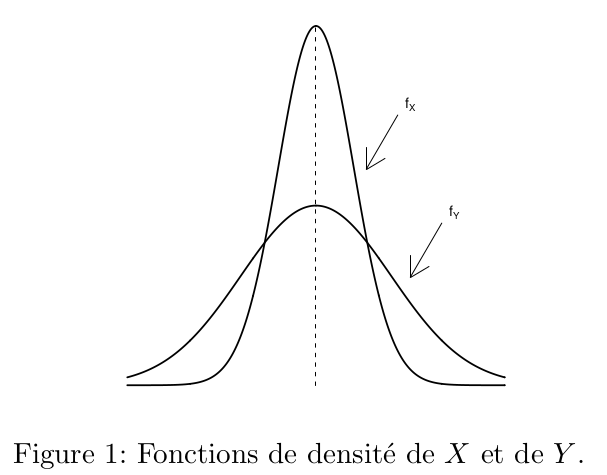
\includegraphics[width=8cm]{ex5.png}
  \\En n’effectuant aucun calcul, l’écart-type de X est-il plus grand que celui de Y ?
  }
  L'écart type est plus grand dans la figure x car les données sont plus écartées que dans la figure y
\end{exo}

	
	
	%
	% Footer
	%
	\vfill
	\hrule
	\vspace{2mm}
	\noindent {\tiny Corrigé Etudiant - TIC} \hfill {\tt \tiny \today}
\end{document}
